\subsection{Fator $\gamma$ do ar: Método de Clément – Desormes}

Para esse primeiro experimento, já explicado na seção anterior, buscaremos encontrar o coeficiente $\gamma$ do ar utilizando o método de Clément -  Desormes. O esquema dos passos que seguiremos está logo abaixo:

\begin{figure}[H]
  \centering
  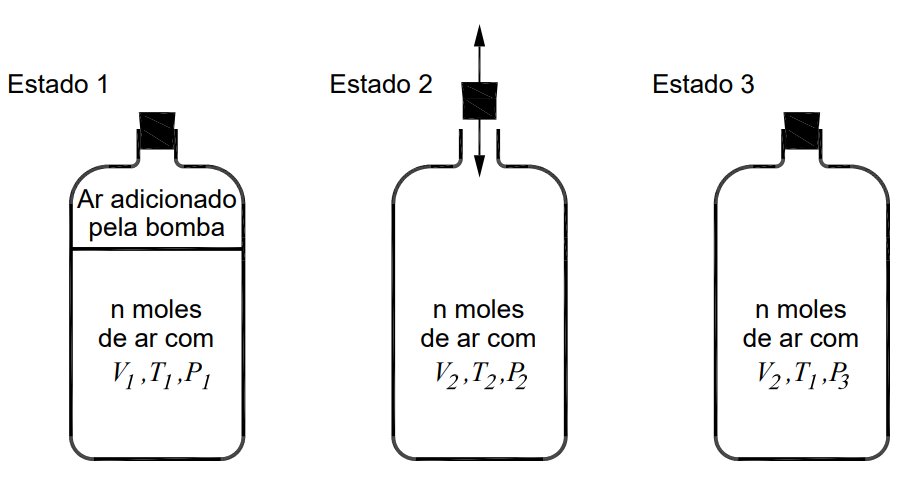
\includegraphics[scale=0.67]{images/Esquema exp.png}
  \caption{Esquema dos três estados que consideramos no processo experimental de Clément-Desormes.}
\end{figure}

Os 3 estados presentes no esquema acima, representam os pontos destacados na Figura \ref{fig:processo-grafico}. Assim, tendo explicitado nosso experimento, podemos dar iniciá-lo.

Primeiramente, vamos tampar a garrafão e bombear manualmente uma certa quantidade de ar para dentro dele, para aumentar a pressão interna. Olhando para o manômetro, esperaremos que o sistema se estabilize - à temperatura ambiente $T_1$ e uma dada pressão $P_1$ (a utilizaremos em função da diferença de altura $h_1$ lida no manômetro).
Chamaremos essa configuração de Estado Inicial ou Estado 1.

Com base na observação do vídeo do experimento, podemos dizer que a altura $h_1$ é a diferença de altura da coluna maior para a menor:\ 
\ \[h_1 = h_{maior} - h_{menor} \]
\[\therefore h_1 = 223,2 cm - 205,2 cm  =  18,0 cm\]
A incerteza de $h_1$ será:\\
\[\delta h_1 = 0,1 cm + 0,1 cm =  0,2 cm\]
\[\therefore h_1 = 18,0 \pm 0,2 cm\]


\begin{figure}[H]
  \centering
  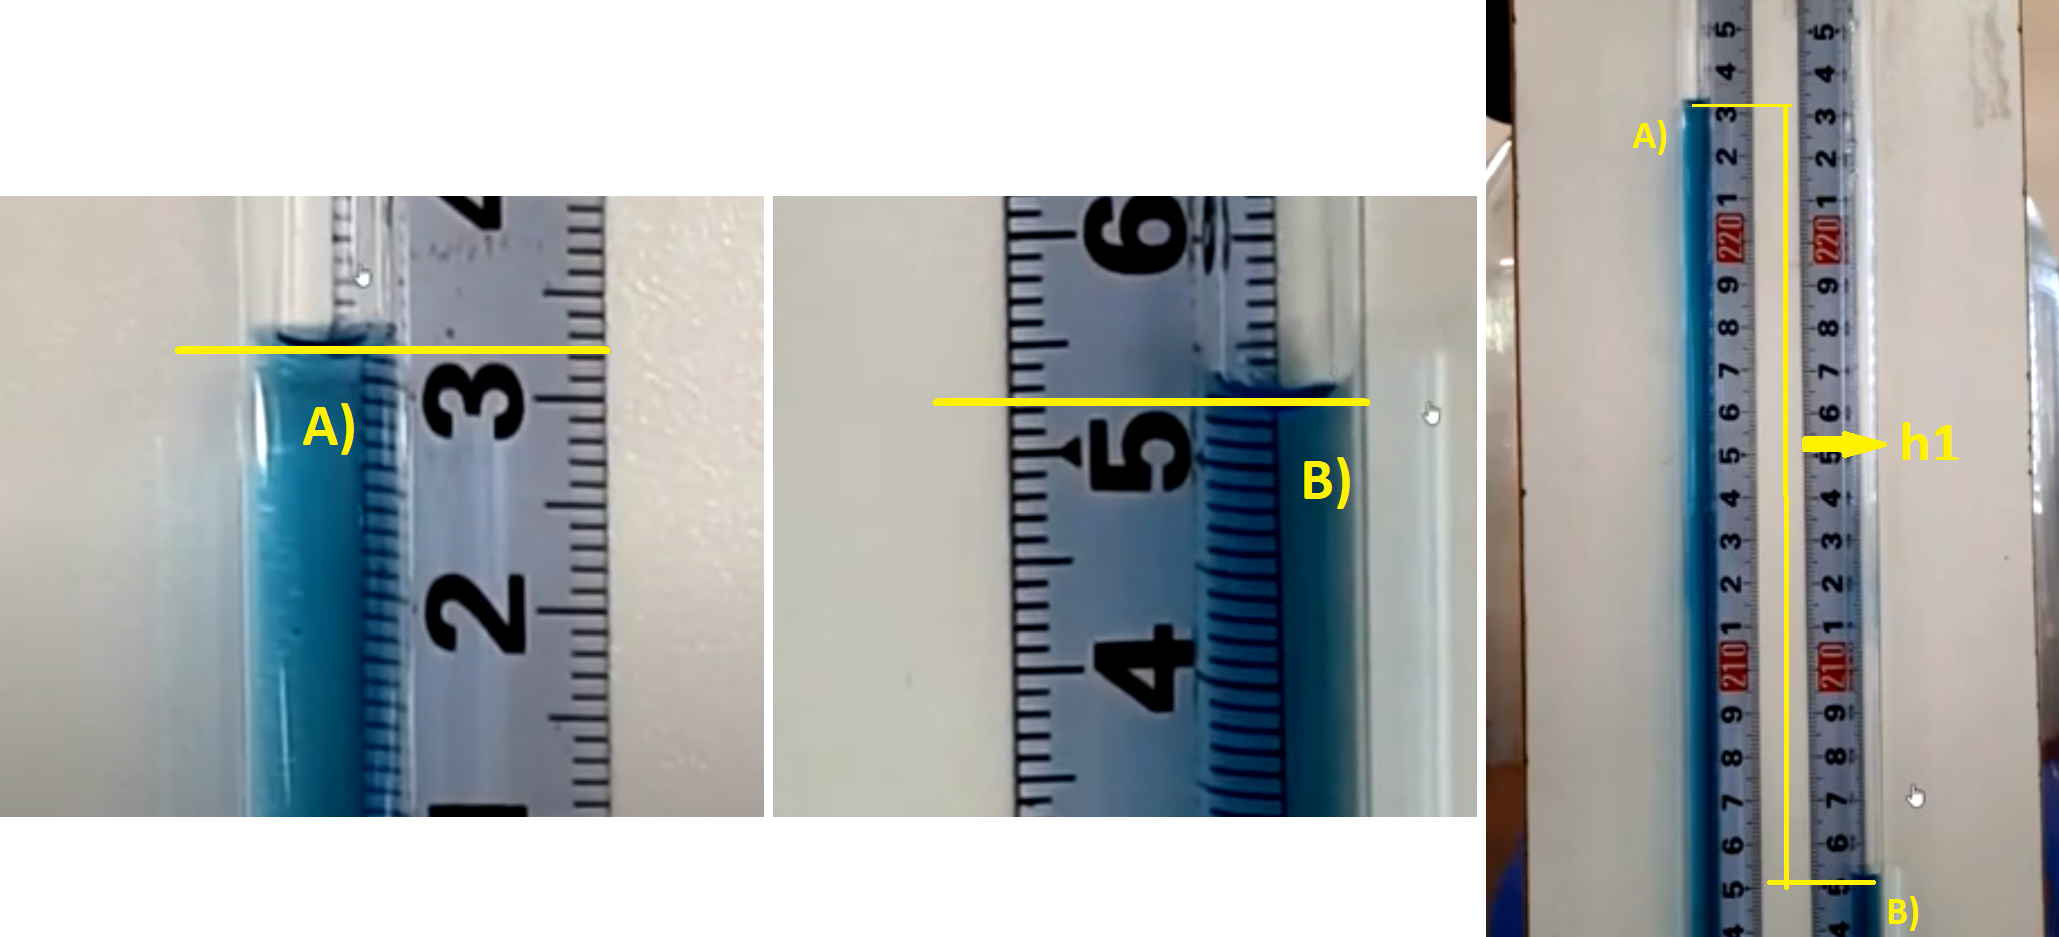
\includegraphics[scale=0.37]{images/Medida 1.1.png}
  \caption{Medida da altura $h_1$ no manômetro (1°experimento).}
\end{figure}

Agora, vamos abrir e fechar a válvula do garrafão. Dessa forma, a pressão interna deve se igualar à pressão atmosférica ($P_2$ = $P_{atm}$). O processo de abrir e fechar o sistema é muito rápido, assim, o gás não tem tempo de trocar calor com o ambiente nesse curto período de tempo, além disso, o vidro do garrafão é um péssimo condutor de calor. Logo, podemos considerar esse processo como adiabático. Ao fechar o tampão da garrafa, chegamos ao Estado Intermediário ou Estado 2, da Figura \ref{fig:processo-grafico}.\\

Logo após a expansão adiabática ocorrer, o gás deve estar em uma temperatura $T_2$ ligeiramente menor que a temperatura ambiente $T_{amb}$ = $T_1$. Após um tempo, a temperatura do sistema irá aumentar e se igualar à temperatura ambiente $T_1$. As paredes rígidas do garrafão garantem que o processo ocorra a volume constante $V_2$ (processo isocórico). Assim que o gás atingir a temperatura $T_1$, estaremos no Estado Final ou Estado 3 pela Figura \ref{fig:processo-grafico}. A pressão nesse ponto ($P_3$) pode ser dada em função da altura $h_3$, que será encontrada a seguir:\

\ \[h_3 = h_{maior} - h_{menor} \]
\[\therefore h_3 = 216,9 cm - 211,3 cm  =  5,6 cm\]
A incerteza de $h_3$ será:\\
\[\delta h_3 = 0,1 cm + 0,1 cm =  0,2 cm\]
\[\therefore h_3 = 5,6 \pm 0,2 cm\]


\begin{figure}[H]
  \centering
  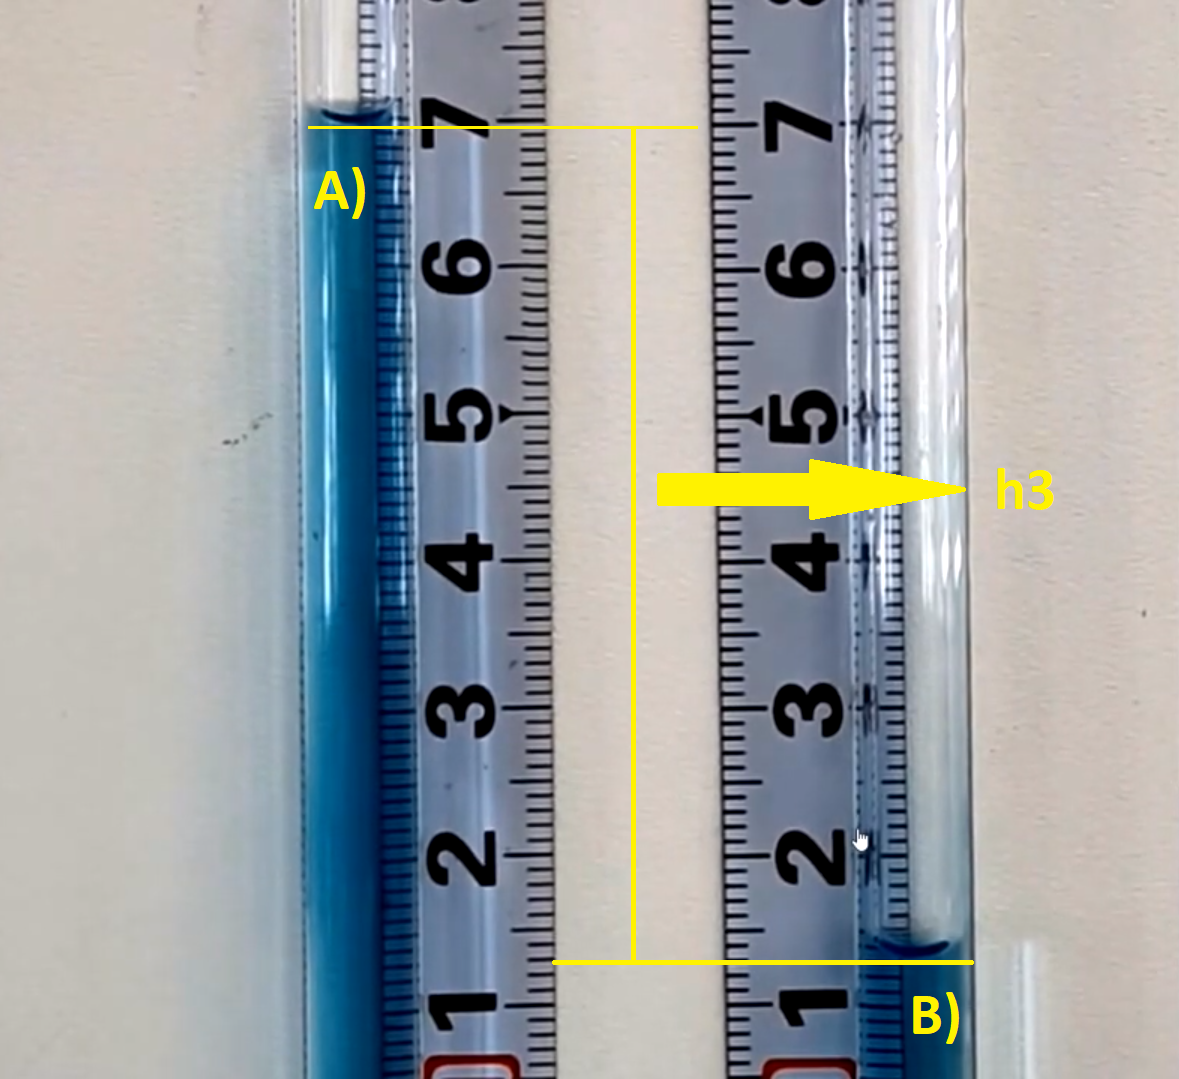
\includegraphics[scale=0.4]{images/Medida 2.1.png}
  \caption{Medida da altura $h_3$ no manômetro (1°experimento).}
\end{figure}

Dessa maneira, conseguimos achar $\gamma$ em função das alturas $h_1$ e $h_3$, como explicitado na seção anterior:\ 

\[ \gamma = \frac{h_1}{h_1 - h_3}\]
\[ \gamma = \frac{18,0}{18,0 - 5,6} = \frac{18,0}{12,4} \]
\[\therefore \gamma = 1,4516129 \approx 1,45\]
E a incerteza de $\gamma$ será:\\
\[\delta \gamma = \frac{(\delta h_1 \cdot h_1 - h_3)+((\delta h_1) + \delta h_3)) \cdot h_1)}{(h_1 - h_3)^2}\]
\[\delta \gamma = \frac{(0,1 \cdot 12,4)+(0,2 \cdot 18,0)}{(12,4)^2}\]
\[\delta \gamma = \frac{4,84}{153,76} = 0,0314776 \approx 0,03\]
Logo:\\ 
\[\therefore \gamma_1 = 1,45 \pm 0,03 \]

Agora, vamos repetir todo esse processo mais duas vezes para poder calcular média e desvio padrão dos nossos valores para o coeficiente $\gamma$, e assim, obter um resultado mais satisfatório.

Na segunda medição, chegamos ao Estado 1 novamente, e medimos nosso $h_1$ - nas mesmas condições que da primeira vez -, que agora ficou:\\

\ \[h_1 = h_{maior} - h_{menor} \]
\[\therefore h_1 = 222,2 cm - 206,1 cm  =  16,1 cm\]
A incerteza de $h_1$ será:\\
\[\delta h_1 = 0,1 cm + 0,1 cm =  0,2 cm\]
\[\therefore h_1 = 16,1 \pm 0,2 cm\]

\begin{figure}[H]
  \centering
  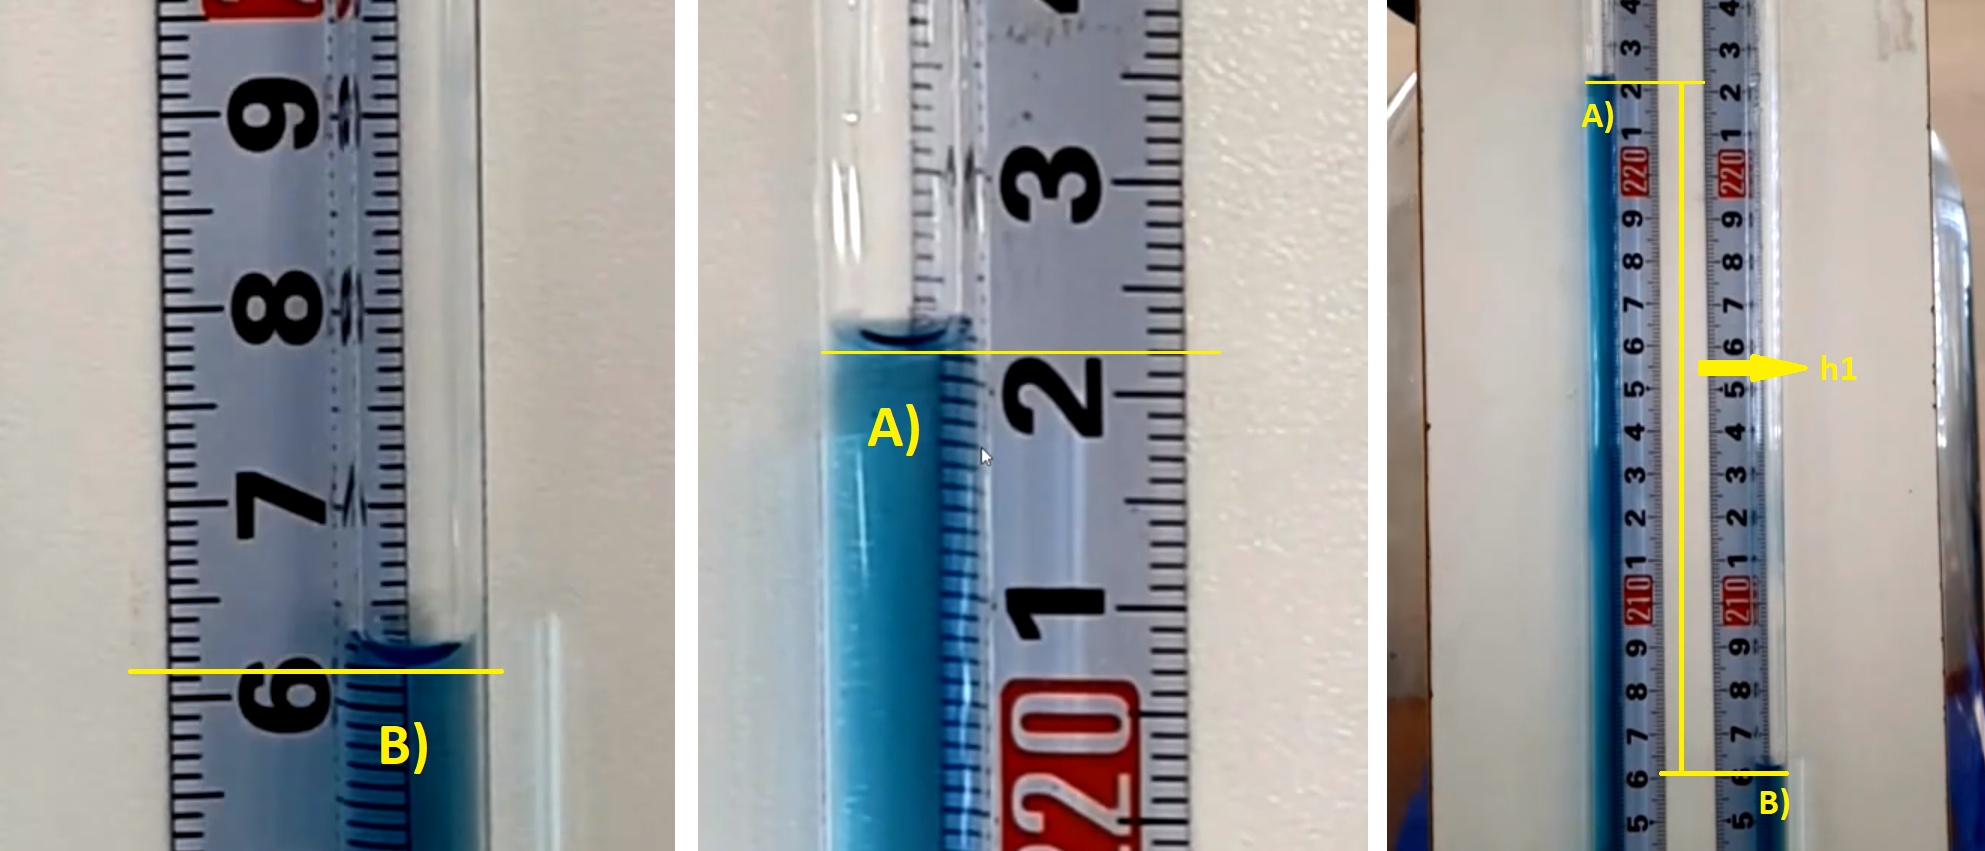
\includegraphics[scale=0.37]{images/Medida 1.2.png}
  \caption{Medida da altura $h_1$ no manômetro (2°experimento).}
\end{figure}

Assim, realizamos o processo adiabático de 1 até 2, e nesse Estado pudemos notar que $T_2$ era menor que $T_1$ e que  $P_2$ = $P_{atm}$, como antes. Depois disso, a temperatura subiu até se igualar à temperatura ambiente $T_1$. Esse processo isocórico, nos leva do Estado 2 para o Estado 3, e a pressão $P_3$ pode ser dada em relação à medida $h_3$ averiguada no manômetro:

\ \[h_3 = h_{maior} - h_{menor} \]
\[\therefore h_3 = 216,1 cm - 212,1 cm  =  4,0 cm\]
A incerteza de $h_3$ será:\\
\[\delta h_3 = 0,1 cm + 0,1 cm =  0,2 cm\]
\[\therefore h_3 = 4,0 \pm 0,2 cm\]


\begin{figure}[H]
  \centering
  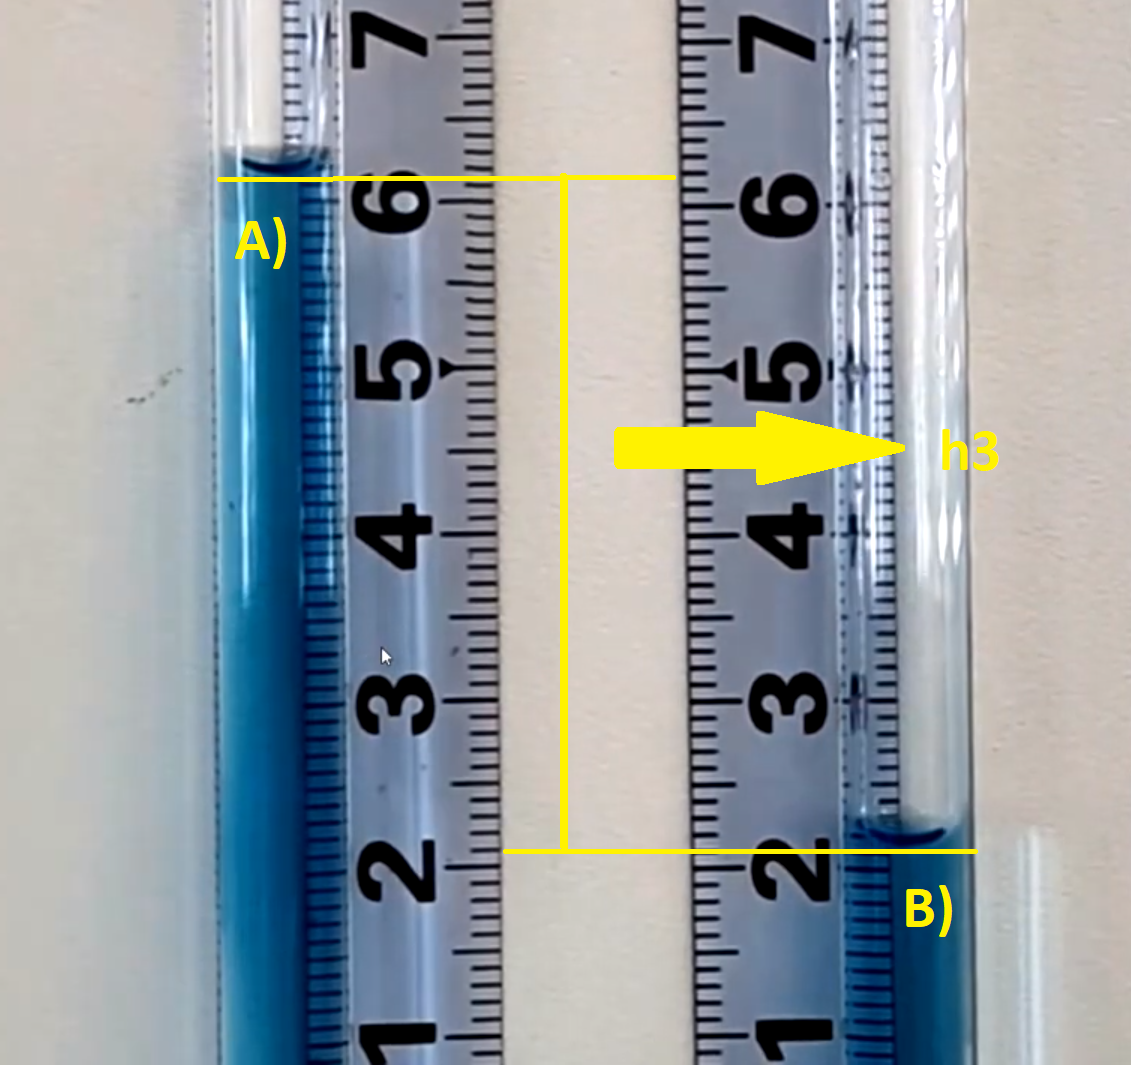
\includegraphics[scale=0.4]{images/Medida 2.2.png}
  \caption{Medida da altura $h_3$ no manômetro (2°experimento).}
\end{figure}

Logo, podemos achar $\gamma$ em função das alturas $h_1$ e $h_3$:\\

\[ \gamma = \frac{h_1}{h_1 - h_3}\]
\[ \gamma = \frac{16,1}{16,1 - 4,0} = \frac{16,1}{12,1} \]
\[\therefore \gamma = 1,3305785 \approx 1,33\]
E a incerteza de $\gamma$ será:\\
\[\delta \gamma = \frac{(\delta h_1 \cdot h_1 - h_3)+((\delta h_1) + \delta h_3)) \cdot h_1)}{(h_1 - h_3)^2}\]
\[\delta \gamma = \frac{(0,1 \cdot 12,1)+(0,2 \cdot 16,1)}{(12,1)^2}\]
\[\delta \gamma = \frac{4,43}{146,41} = 0,0302575 \approx 0,03\]
Logo:\\ 
\[\therefore \gamma_2 = 1,33 \pm 0,03 \]

Por último, faremos as mesmas medidas pela terceira vez, buscando $h_1$ e $h_3$ para o cálculo de $\gamma$, então, vamos apresentar diretamente os valores das alturas, uma vez que o processo já foi explicado acima, e vamos realizá-lo identicamente.\\

No Estado 1, teremos:\\

\ \[h_1 = h_{maior} - h_{menor} \]
\[\therefore h_1 = 223,0 cm - 205,3 cm  =  17,7 cm\]
A incerteza de $h_1$ será:\\
\[\delta h_1 = 0,1 cm + 0,1 cm =  0,2 cm\]
\[\therefore h_1 = 17,7 \pm 0,2 cm\]

\begin{figure}[H]
  \centering
  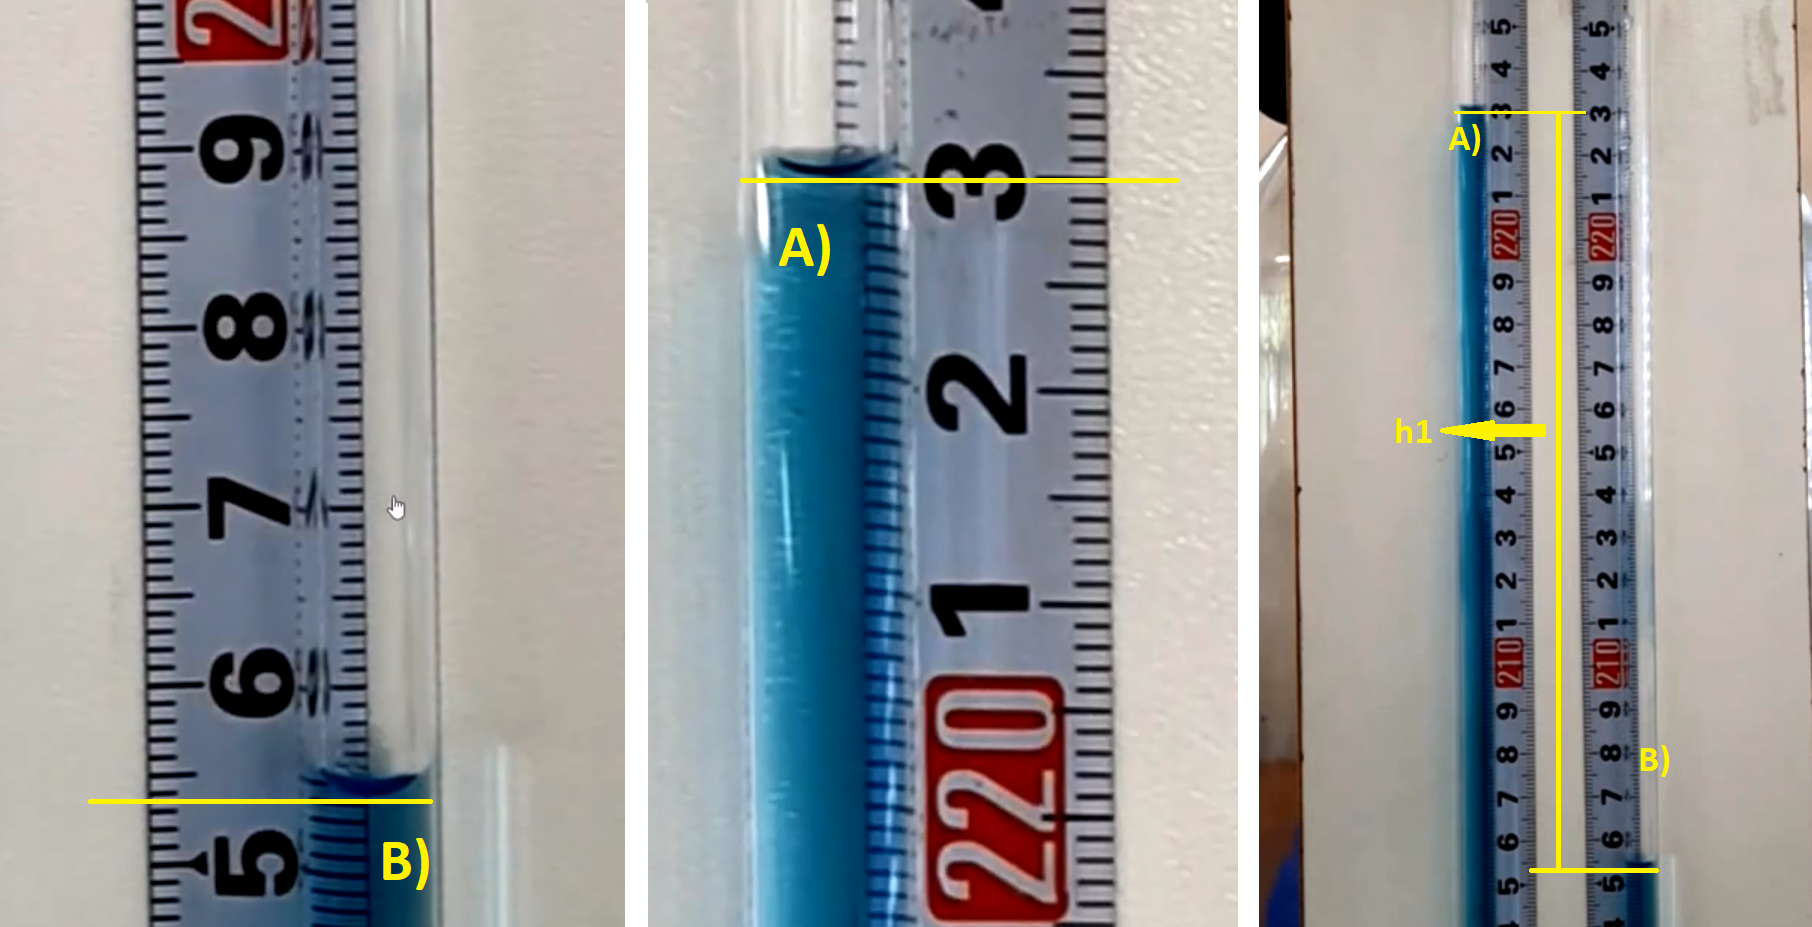
\includegraphics[scale=0.37]{images/Medida 1.3.png}
  \caption{Medida da altura $h_1$ no manômetro (3°experimento).}
\end{figure}

Já para o Estado 3:\\

\ \[h_3 = h_{maior} - h_{menor} \]
\[\therefore h_3 = 216,7 cm - 211,6 cm  = 5,1 cm\]
A incerteza de $h_3$ será:\\
\[\delta h_3 = 0,1 cm + 0,1 cm =  0,2 cm\]
\[\therefore h_3 = 5,1 \pm 0,2 cm\]


\begin{figure}[H]
  \centering
  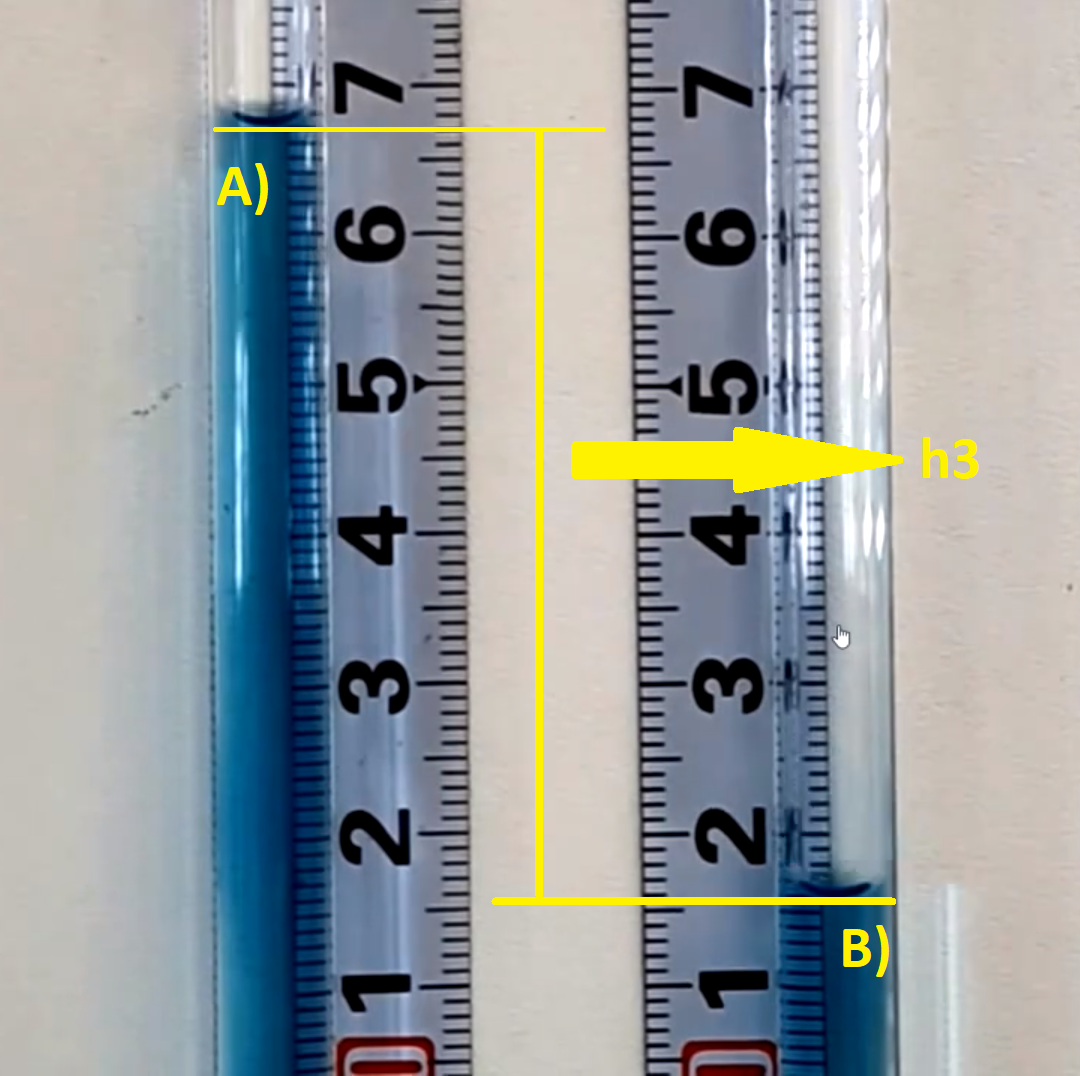
\includegraphics[scale=0.4]{images/Medida 2.3.png}
  \caption{Medida da altura $h_3$ no manômetro (3°experimento).}
\end{figure}

Com as alturas $h_1$ e $h_3$ calculadas, conseguimos obter o coeficiente $\gamma$:\\

\[ \gamma = \frac{h_1}{h_1 - h_3}\]
\[ \gamma = \frac{17,7}{17,7 - 5,1} = \frac{17,7}{12,6} \]
\[\therefore \gamma = 1,4047619 \approx 1,40 \]
E a incerteza de $\gamma$ será:\\
\[\delta \gamma = \frac{(\delta h_1 \cdot h_1 - h_3)+((\delta h_1) + \delta h_3)) \cdot h_1)}{(h_1 - h_3)^2}\]
\[\delta \gamma = \frac{(0,1 \cdot 12,6)+(0,2 \cdot 16,1)}{(12,6)^2}\]
\[\delta \gamma = \frac{4,48}{158,76} = 0,02821869 \approx 0,03\]
Logo:\\ 
\[\therefore \gamma_3 = 1,40 \pm 0,03 \]

Assim, até agora obtivemos os seguintes valores para $\gamma$ nos 3 experimentos analisados:\\

\begin{table}[H]
    \centering
    \begin{tabular}{ |c||c||c| }
        \hline
        \textbf{Número do experimento} & \textbf{Valor} & \textbf{Incerteza}\\
        \hline 
        1º experimento ($\gamma_1$)       & 1,45   & 0,03  \\
        2º experimento ($\gamma_2$)       & 1,33   & 0,03  \\
        3º experimento ($\gamma_3$)       & 1,40   & 0,03  \\
        \hline
        \end{tabular}
    \caption{Valores de $\gamma$ para cada um dos experimentos realizados} 
\end{table}


Tendo esses valores, podemos então calcular a média e o desvio padrão desses resultados.\\

A média $\overline{\gamma}$ será dada por:

\[ \overline{\gamma} = \frac{\sum_{i=1}^{N} \gamma_i}{N}\]
\[ \overline{\gamma} = \frac{\sum_{i=1}^{3} \gamma_i}{3}\]
\[ \overline{\gamma} = \frac{(1,45) + (1,33) + (1,40)}{3}\]
\[ \overline{\gamma} = 1,3933333333 \approx 1,39\]

E sua incerteza será:\\
\[ \delta\overline{\gamma} = \frac{\sum_{i=1}^{N} |\gamma_i - \overline{\gamma}|}{N}\]
\[ \delta\overline{\gamma} = \frac{\sum_{i=1}^{3} |\gamma_i - \overline{\gamma}|}{3}\]
\[ \delta\overline{\gamma} = \frac{(|1,45 - 1,39|) + (|1,33 - 1,39|) + (|1,40 -1,39|) }{3}\]
\[ \delta\overline{\gamma} = \frac{0,13}{3} = 0,043333333 \approx 0,04\]

Logo, $\gamma$ pode ser representado, de forma menos rigorosa, por:
\[ \overline{\gamma} \pm \delta  = 1,39 \pm 0,04 \]

Já o desvio padrão $\sigma$, é dado por:

\[ \sigma = \sqrt{\frac{\sum_{i=1}^{N} (\gamma_i - \overline{\gamma})^2}{N-1}}\]
\[ \sigma = \sqrt{\frac{\sum_{i=1}^{3} (\gamma_i - \overline{\gamma})^2}{2}}\]
\[ \sigma = \sqrt{\frac{(1,45-1,39)^2 + (1,33-1,39)^2 + (1,40-1,39)^2}{2}}\]
\[ \sigma = \sqrt{\frac{0,0036 + 0,0036 + 0,0001}{2}}\]
\[ \sigma = \sqrt{\frac{0,0073}{2}} = \sqrt{0,00365} \]
\[ \therefore \sigma = 0,06041523 \approx 0,06 \]

Então o resultado do experimento com sua incerteza deve ser representado da seguinte forma:
\[ \overline{\gamma} \pm \sigma = 1,39 \pm 0,06\]\\

Agora, faremos algumas deduções de fórmulas que foram utilizadas por nós ao longo do experimento. Primeiramente, vamos deduzir a primeira relação que chegamos para o coeficiente $\gamma$:

Com base no gráfico da Figura \ref{fig:processo-grafico}, vamos considerar a relação entre $P$ e $V$ no decorrer do processo adiabático explicitado no gráfico. 
Sabemos que $P V^\gamma = cte $, logo, no processo adiabático, podemos dizer que:\\
\[P_1 V_1^\gamma = P_2 V_2^\gamma\]
Assim, temos que:
\[\frac{V_1^\gamma}{V_2^\gamma}  = \frac{P_2}{P_1}\]
\[\left(\frac{V_1}{V_2}\right)^\gamma  = \left(\frac{P_2}{P_1}\right)\]\\
Como queremos analisar o coeficiente $\gamma$ e ele aparece no expoente, podemos aplicar o logaritmo natural dos dois lados da equação, teremos:\\
\[\gamma \ln\left(\frac{V_1}{V_2}\right)  = \ln \left(\frac{P_2}{P_1}\right)\]\\
Isolando o coeficiente em termos da pressão $P_1$ e $P_2$ e dos volumes $V_1$ e $V_2$, ficaremos com a seguinte relação:\\
\[\gamma  = \frac{\ln{\left(\frac{P_2}{P_1}\right)}}{\ln{\left(\frac{V_1}{V_2}\right)}} \]\\ 
Assim obtemos a equação 22, da Apostila de Laboratório (\ref{bibl:apostila}).\\

Outra dedução que faremos, é a da relação final que usamos para achar $\gamma$ em função das alturas:\\

Da equação 22 podemos utilizar a passagem já explicada na seção Materiais e Métodos, para provar que:
\[ \gamma = \frac{ln\frac{P_2}{P_1}}{ln\frac{V_1}{V_2}} \ \ = \ \ \frac{ln\frac{P_2}{P_1}}{ln\frac{P_3}{P_1}} \] \

Desse modo, conhecendo as pressões:

\[ P_1 = P_{atm} + \rho g h_1 \]
\[ P_2 = P_{atm} \]
\[ P_3 = P_{atm} + \rho g h_3 \] \

Podemos obter:
\[ P_1 = P_{atm}\left( 1+\frac{\rho g h_1}{P_{atm}}\right) \ \  e  \ \ P_3 = P_{atm}\left(1+\frac{\rho g h_3}{P_{atm}}\right) \]\\

Substituindo os valores das pressões podemos dizer que $\gamma$ é:\\
\[ \gamma = \frac{ln\left(\frac{P_{atm}}{P_{atm}+\rho g h_1}\right) }{ln\left (\frac{P_{atm}+\rho g h_3}{P_{atm}+\rho g h_1}\right) } = \frac{ln\left(\frac{P_{atm}}{P_{atm}(1 + \rho g h_1)}\right) }{ln\left (\frac{P_{atm} ( 1 + \rho g h_3)}{P_{atm} ( 1 + \rho g h_1)}\right) } \]

\[ \gamma = \frac{ln\left(\frac{1}{1 + \rho g h_1}\right)}{ln\left (\frac{1 + \rho g h_3}{ 1 + \rho g h_1}\right) }  =  \frac{\ln{1}-\ln{(1+\rho g h_1}}{\ln{1+ \rho g h_3)} - \ln{(1+\rho g h_1)}}\]\\

Assim, como ($ \rho g h << P_{atm}$), podemos assumir que $\ln{\left(1+ \frac{\rho g h}{P_{atm}}\right)} \approx \frac{\rho g h}{P_{atm}} $, como já explicado na seção Materiais e Métodos $^{[MM1]}$. Desse modo:\\

\[ \gamma = \frac{0 - [(\rho g h_1) \cdot (-1)]}{[(\rho g h_3) - (\rho g h_1)] \cdot (-1)}\]

\[ \gamma = \frac{(\rho g h_1)}{(\rho g h_1) - (\rho g h_3)} = \frac{h_1}{h_1 - h_3}\] \\

Então, demonstramos agora a equação (28) da Apostila de Laboratório (\ref{bibl:apostila}).\\

Desse modo, realizamos o experimento e ainda deduzimos as equações (22) e (28) utilizadas na prática. \\
